\begingroup
\clearpage% Manually insert \clearpage
\let\clearpage\relax% Remove \clearpage functionality
\vspace*{-16pt}% Insert needed vertical retraction
\chapter[THE STANDARD MODEL OF PARTICLE PHYSICS]{THE STANDARD MODEL OF PARTICLE PHYSICS}
\endgroup

% ============================================================
% MASTER TODO LIST FOR THIS CHAPTER
% ------------------------------------------------------------
% PROSE TO WRITE:
%   [ ] Section 2.2 — Higgs Mechanism (currently bullet points)
%   [ ] Section 2.3 — Yukawa Couplings (currently bullet points)
%   [ ] Section 2.4 — Rewrite opening paragraph (duplicates Sec 2.2)
%   [ ] Section 2.4 — Convert bottom bullet points to prose
%   [ ] Section 2.5 — Open Questions (currently bullet points)
%
% FIGURES:
%   [ ] fig:HiggsProduction    — add caption (see TODO comment inline)
%   [ ] fig:HiggsBranchingRatios — add caption (see TODO comment inline)
%
% BIB ENTRIES NEEDED (cite keys used in text, not yet in references.bib):
%   [ ] PDG2022          — Workman et al., PTEP 2022, 083C01
%   [ ] Peskin:1995ev    — Peskin & Schroeder, QFT textbook (1995)
%   [ ] ATLASHiggsTenYears / fix key — arXiv:2207.00092
%   [ ] ATLASDiscovery   — arXiv:1207.7214
%   [ ] CMSDiscovery     — arXiv:1207.7235
%   [ ] LHCHiggsXSWG4   — arXiv:1610.07922
%   [ ] Buttazzo:2013uya — arXiv:1307.3536
% ============================================================

% ============================================================
% REFERENCES FOR THIS CHAPTER
% ------------------------------------------------------------
% PDG Review of Particle Physics: Workman et al., PTEP 2022, 083C01
%   https://pdg.lbl.gov
% Glashow electroweak: Nucl. Phys. 22, 579 (1961)
% Weinberg electroweak unification: PRL 19, 1264 (1967)
%   https://arxiv.org/abs/... [no arXiv; DOI: 10.1103/PhysRevLett.19.1264]
% Englert & Brout (SSB): PRL 13, 321 (1964)
%   DOI: 10.1103/PhysRevLett.13.321
% Higgs PRL letter: PRL 13, 508 (1964)
%   DOI: 10.1103/PhysRevLett.13.508
% Guralnik, Hagen & Kibble: PRL 13, 585 (1964)
%   DOI: 10.1103/PhysRevLett.13.585
% kappa-framework (LHC Higgs XS WG Yellow Report 3): arXiv:1307.1347
% LHC Higgs XS WG Yellow Report 4: arXiv:1610.07922
% ATLAS Higgs discovery: arXiv:1207.7214
% CMS Higgs discovery: arXiv:1207.7235
% ATLAS Run 2 coupling combination: arXiv:2207.00116
% ATLAS Nature Higgs summary (10 years): arXiv:2207.00092
% EW vacuum stability (Degrassi et al.): arXiv:1205.6497
% Peskin & Schroeder, An Introduction to Quantum Field Theory,
%   Addison-Wesley (1995), Chapter 4 -- gauge invariance, covariant derivative
%   cite key: Peskin:1995ev
% ============================================================

% ============================================================
% SECTION 2.1 — THE STANDARD MODEL
% ------------------------------------------------------------
% OPENS WITH: What is the theoretical framework underlying all
%             known fundamental interactions?
% LEAVES OPEN: The SM gauge symmetry forbids explicit mass terms
%              for W, Z bosons and fermions. How does nature
%              generate these masses while preserving gauge invariance?
% ============================================================

\section{The Standard Model}

The Standard Model (SM) is the theoretical framework that describes all
known fundamental particles and three of the four fundamental forces of
nature. The SM organizes its particles into two broad categories: fermions and bosons.
Fermions are particles with half-integer spin and make up the matter
content of the universe. Bosons are particles with integer spin and
are responsible for mediating the fundamental forces.

The fermions are divided into two families: quarks and leptons, each
arranged into three generations of increasing mass. The first generation
contains the lightest and most stable particles: the up and down quarks,
the electron, and the electron neutrino. The second and third generations
are heavier copies with otherwise identical quantum numbers. All ordinary
matter is composed of first-generation particles, and the heavier
generations are unstable and decay to first-generation particles. Why
nature repeats this pattern exactly three times is not predicted by the SM
and remains an open question.
Quarks carry electric charge, weak charge, and color charge, and therefore
interact with all three SM forces. Quarks are never observed in isolation
and are always found confined inside composite particles called hadrons,
such as the proton ($uud$) and neutron ($udd$). The leptons follow the
same three-generation pattern, with the electron, muon, and tau each
paired with a corresponding neutrino. Leptons carry electric and
weak charge but no color charge. Neutrinos carry only weak charge and
interact exclusively through the weak force.

The force carriers are spin-1 gauge bosons. The massless photon mediates the
electromagnetic force. The $W^\pm$ and $Z$ bosons mediate
the weak force and are massive, at 80 and 92 GeV, respectively. Eight massless gluons mediate the strong force. The Higgs boson is distinct from the gauge bosons as it is the
only spin-0 fundamental particle and does not mediate a force. Instead it
plays a central role in mass generation, as described in
Section~\ref{sec:higgs_mechanism}. The Standard Model is shown in
Figure~\ref{fig:SM}.

\begin{figure}[h]
	\centering
	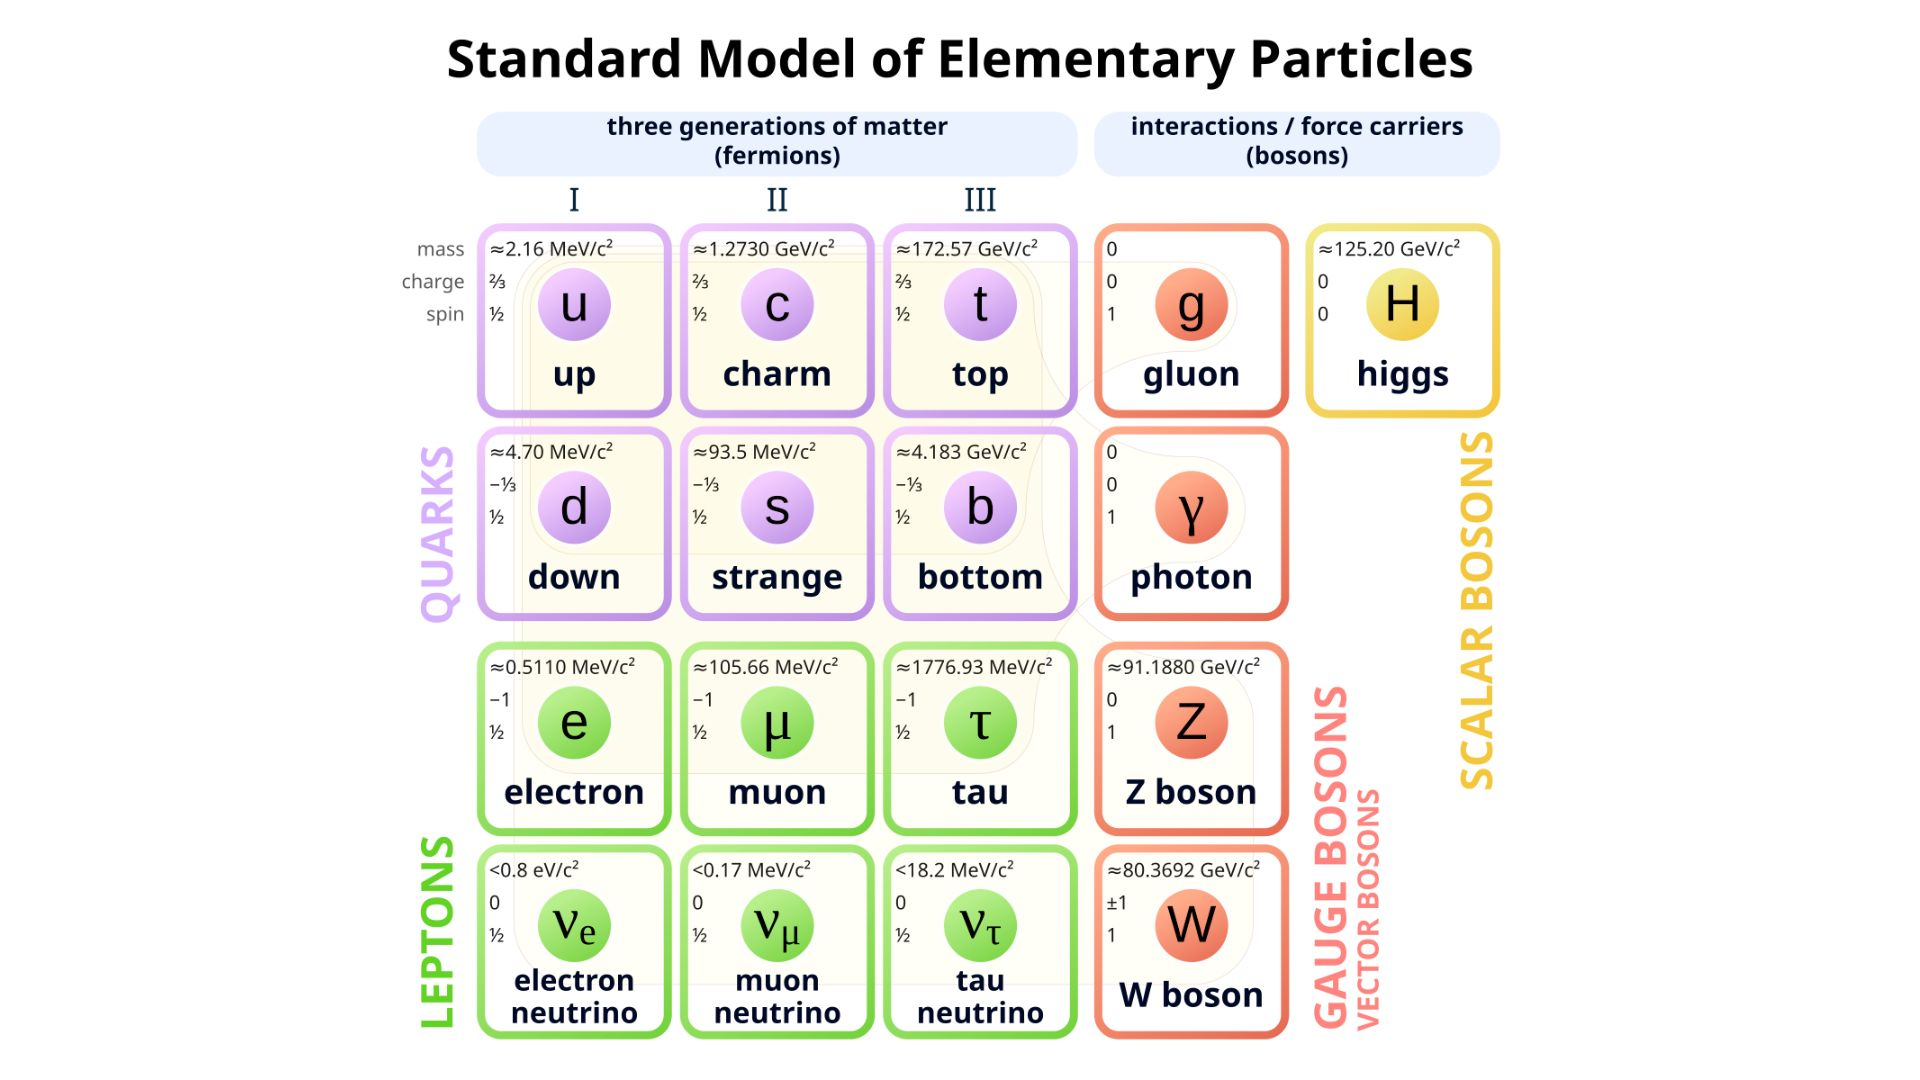
\includegraphics[width=0.85\linewidth]{figures/chapter2/SM.jpg}
	\caption{The fundamental particles organized by generation and type.}
	\label{fig:SM}
\end{figure}

In essence, the SM is a theory explaining the underlying symmetries of
nature. A symmetry in physics is an invariance under some transformation.
A classical example is translational symmetry, in which the outcome of an
experiment does not depend on where in space it is performed. In the SM,
the relevant symmetries are gauge symmetries, also called local symmetries.
To understand the distinction between a global and a local symmetry,
consider an analogy. Imagine a vector field $\vec{\psi}(x)$ spread across
space, each pointing in some direction. A global symmetry $\alpha$ is like
rotating every vector by the same fixed angle simultaneously,
$\vec{\psi}(x) \rightarrow \alpha \cdot \vec{\psi}(x)$. The relative
relationships between all vectors are preserved, and the physics is
unchanged. A gauge, or local, symmetry $\alpha(x)$ is more constraining.
Each vector is allowed to be rotated by a different angle at each point in
space independently, $\vec{\psi}(x) \rightarrow \alpha(x) \cdot \vec{\psi}(x)$.
In the language of quantum field theory, this corresponds to a local phase
rotation of the fermion field~\cite{Peskin:1995ev}:
\begin{equation}
    \psi(x) \rightarrow e^{i\alpha(x)}\psi(x).
    \label{eq:U1_gauge_transform}
\end{equation}
For the physics to remain consistent under this position-dependent
transformation, a new field $A_\mu(x)$ must be introduced to compensate
for the varying phase from point to point. This is achieved by replacing
the ordinary derivative $\partial_\mu$ with the covariant derivative,
\begin{equation}
    D_\mu = \partial_\mu + igA_\mu(x),
    \label{eq:covariant_derivative}
\end{equation}
where $g$ is the coupling strength. The field $A_\mu$ is precisely a gauge
boson. In this way, the forces of nature emerge as a direct consequence of
demanding local gauge invariance.

The SM is invariant under the gauge symmetry group
$\text{SU}(3)_C \times \text{SU}(2)_L \times \text{U}(1)_Y$. Each factor
corresponds to one of the SM forces. The $\text{SU}(3)_C$ symmetry governs
the strong force, with the subscript $C$ denoting color charge. Its eight
generators correspond to the eight gluons. The
$\text{SU}(2)_L \times \text{U}(1)_Y$ symmetry governs the electroweak
force, with $L$ indicating that the weak interaction acts only on
left-handed fermions and $Y$ denoting hypercharge. Together these produce
four gauge bosons: the $W^+$, $W^-$, $W^0$, and $B^0$. After electroweak
symmetry breaking, these mix to form the physical $W^\pm$, $Z$, and
$\gamma$.

The dynamics of all SM particles and their interactions are encoded in the
SM Lagrangian density~\cite{PDG2022}:

\begin{equation}
  \mathcal{L}_{SM} =
  \underbrace{-\frac{1}{4}F^{a}_{\mu\nu}F^{a\mu\nu}}_{\text{gauge kinetic}}
  + \underbrace{i\bar{\psi} \gamma^\mu D_\mu \psi}_{\text{fermion kinetic}}
  + \underbrace{|D_\mu\phi|^2 - V(\phi)}_{\text{Higgs sector}}
  + \underbrace{y_{ij}\bar{\psi}_{Li}\phi\psi_{Rj} + \text{h.c.}}_{\text{Yukawa}}
  \label{eq:SMlagrangian}
\end{equation}
% Note on indices:
% F^a_{\mu\nu}: a = gauge group generator index (summed over SU(3), SU(2), U(1)); mu,nu = Lorentz indices
% psi: implicit sum over all fermion flavors; mu = Lorentz index on gamma matrix
% D_mu phi: covariant derivative of Higgs doublet; |...|^2 = (D_mu phi)^dag (D^mu phi)
% y_{mn}: 3x3 Yukawa matrix; m,n = generation indices (chosen to avoid clash with imaginary unit i)
% Reference: PDG Review, Workman et al. PTEP 2022, 083C01 (Electroweak Model chapter)

The gauge kinetic term $-\frac{1}{4}F^a_{\mu\nu}F^{a\mu\nu}$ describes
how the gauge fields propagate and self-interact. The field strength tensor
$F^a_{\mu\nu}$ encodes the derivatives and self-couplings of each gauge
field. The fermion kinetic term $i\bar{\psi}\gamma^\mu D_\mu\psi$ describes
how fermions propagate and interact with the gauge fields. The ordinary
derivative is replaced by the covariant derivative $D_\mu$, which
automatically inserts the correct interaction vertex between a fermion and
a gauge boson. This substitution is the mathematical implementation of
local gauge invariance. The Higgs sector $|D_\mu\phi|^2 - V(\phi)$
describes the Higgs field, its self-interaction potential, and its
couplings to the gauge bosons. The potential $V(\phi)$ drives the
spontaneous symmetry breaking discussed in
Section~\ref{sec:higgs_mechanism}. Finally, the Yukawa term
$y_{ij}\bar{\psi}_{Li}\phi\psi_{Rj}$ couples the fermions to the Higgs
field. After symmetry breaking, this term generates the fermion masses
discussed in Section~\ref{sec:yukawa}.

Despite its precision, the SM does not describe gravity, does not account
for dark matter or dark energy, and provides no explanation for the
observed matter-antimatter asymmetry of the universe. These open questions
are discussed in Section~\ref{sec:open_questions}.
% References: PDG (Workman et al. 2022), Glashow 1961, Weinberg 1967

\newpage

% ============================================================
% SECTION 2.2 — THE HIGGS MECHANISM
% ------------------------------------------------------------
% ANSWERS: The SM gauge symmetry forbids explicit mass terms.
%          The Higgs mechanism generates masses dynamically
%          through spontaneous symmetry breaking.
% LEAVES OPEN: The Higgs mechanism predicts a new scalar boson.
%              Has it been observed? What are its properties?
% ============================================================

\section{The Higgs Mechanism}
\label{sec:higgs_mechanism}

% ------------------------------------------------------------
% OUTLINE FOR THIS SECTION:
% Para 1 — The mass problem
%   - SM gauge invariance forbids explicit mass terms for W, Z
%   - Explicit m_W^2 W_mu W^mu breaks gauge invariance
%   - Yet W (~80 GeV) and Z (~91 GeV) are observed to be massive
% Para 2 — The Higgs potential and spontaneous symmetry breaking
%   - Introduce complex scalar doublet phi with V(phi) = mu^2|phi|^2 + lambda|phi|^4
%   - For mu^2 < 0: unstable at origin, degenerate ring of minima at |phi| = v/sqrt(2)
%   - v ~ 246 GeV is the vacuum expectation value
%   - Field settles into one minimum: SSB of SU(2)_L x U(1)_Y -> U(1)_EM
%   - Reference figure: Higgs potential (fig:HiggsPotential)
% Para 3 — Consequences of SSB: gauge boson masses and the Higgs boson
%   - Three broken generators -> three Goldstone bosons
%   - Goldstone bosons absorbed by W+, W-, Z -> longitudinal modes -> mass
%   - Photon corresponds to unbroken generator -> remains massless
%   - Remaining physical DOF: real scalar Higgs boson h
%   - Optional: show W and Z mass formulae m_W = gv/2, m_Z = sqrt(g^2+g'^2)v/2
% ------------------------------------------------------------

\begin{itemize}
  \item A complex scalar doublet $\phi$ with potential $V(\phi) = \mu^2|\phi|^2 + \lambda|\phi|^4$ is introduced. For $\mu^2 < 0$, the minimum is a degenerate circle at $|\phi| = v/\sqrt{2}$, where $v \approx 246$ GeV is the vacuum expectation value.
  \item The ground state spontaneously selects one minimum, breaking $\text{SU}(2)_L \times \text{U}(1)_Y \rightarrow \text{U}(1)_{EM}$. Three Goldstone bosons are absorbed by the $W^{\pm}$ and $Z$, giving them mass. The photon remains massless.
  \item The remaining degree of freedom is the Higgs boson $h$, a real scalar representing oscillations about the minimum.
  % W and Z masses arise from |D_mu phi|^2 after SSB:
  %   m_W = \frac{1}{2} g v, \qquad m_Z = \frac{1}{2}\sqrt{g^2 + g'^2}\, v
  % where g, g' are the SU(2)_L and U(1)_Y couplings. With v = 246 GeV: m_W ~ 80 GeV, m_Z ~ 91 GeV.
  % References: Englert & Brout PRL 1964, Higgs PRL 1964, Guralnik/Hagen/Kibble PRL 1964
\end{itemize}

\begin{figure}[h]
	\centering
	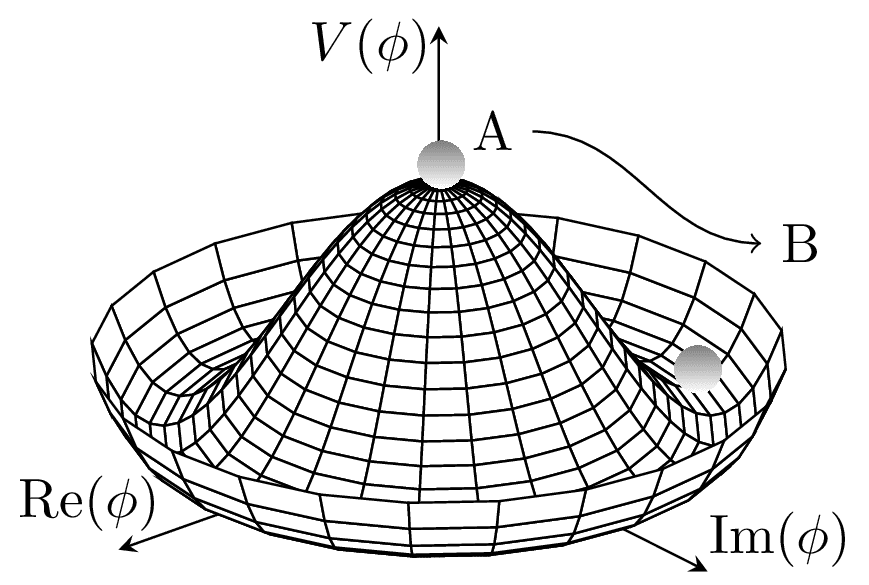
\includegraphics[width=0.5\linewidth]{figures/chapter2/higgs_potential.png}
	\caption{The Higgs potential $V(\phi) = \mu^2|\phi|^2 + \lambda|\phi|^4$ for $\mu^2 < 0$.
	Point A is the unstable maximum at $\phi = 0$. Point B is a stable minimum at $|\phi| = v/\sqrt{2}$.
	The ground state spontaneously selects one minimum, breaking $\text{SU}(2)_L \times \text{U}(1)_Y \rightarrow \text{U}(1)_\text{EM}$.}
	\label{fig:HiggsPotential}
\end{figure}

\newpage

% ============================================================
% SECTION 2.3 — YUKAWA COUPLINGS AND FERMION MASS GENERATION
% ------------------------------------------------------------
% ANSWERS: The Higgs mechanism gives mass to gauge bosons.
%          Yukawa couplings extend this to give mass to fermions.
% LEAVES OPEN: Yukawa couplings are free parameters in the SM.
%              Are the observed coupling strengths consistent with
%              SM predictions? Are second-generation couplings
%              (charm, muon) accessible at the LHC?
% ============================================================

\section{Yukawa Couplings and Fermion Mass Generation}
\label{sec:yukawa}

% ------------------------------------------------------------
% OUTLINE FOR THIS SECTION:
% Para 1 — Fermion mass generation via Yukawa interactions
%   - Gauge invariance also forbids explicit fermion mass terms before SSB
%   - Yukawa term: L_Y = -y_f psi_L phi psi_R + h.c.
%   - After SSB: m_f = y_f * v / sqrt(2)
%   - Key SM prediction: Higgs coupling to any fermion proportional to its mass
% Para 2 — Experimental status of Yukawa couplings
%   - Third-generation (t, b, tau) measured, consistent with SM
%   - Top quark special: m_t ~ 173 GeV -> y_t ~ 1, strongest Higgs coupling
%   - Introduce kappa-framework: kappa_f = y_f / y_f^SM as BSM probe
%   - Reference figure: ATLAS coupling vs mass plot (fig:HiggsCouplings)
% Para 3 — Second-generation gap and thesis motivation
%   - Charm and muon Yukawa couplings largely unmeasured
%   - Many BSM models predict enhanced kappa_c
%   - VH(H->cc) analysis in this thesis directly probes y_c
% ------------------------------------------------------------

\begin{itemize}
  \item Yukawa terms $\mathcal{L}_Y = -y_f \bar{\psi}_L \phi \psi_R + \text{h.c.}$ give each fermion a mass $m_f = y_f v/\sqrt{2}$ after SSB. The SM predicts coupling strength proportional to mass.
  % Explicit fermion mass terms are forbidden by gauge invariance before SSB.
  \item Third-generation couplings ($t$, $b$, $\tau$) have been measured and are consistent with the SM. The top quark is the most special case: with $m_t \approx 173$~GeV, its Yukawa coupling is close to unity ($y_t \approx 1$), making it by far the most strongly coupled fermion to the Higgs field. Second-generation couplings ($c$, $\mu$) remain largely untested and are the target of ongoing analyses including this thesis.
  % Deviations from y_f proportional to m_f would be a direct signal of BSM physics.
  %   SOURCE: Figure 5 in ATLAS Nature paper arXiv:2207.00092
  %     DOI: 10.1038/s41586-022-04893-w
  %     "A detailed map of Higgs boson interactions by the ATLAS experiment
  %      ten years after the discovery", Nature 607, 52-59 (2022)
  %   SOURCE (alt): fig_05 from ATLAS paper HIGG-2021-23
  %     https://atlas.web.cern.ch/Atlas/GROUPS/PHYSICS/PAPERS/HIGG-2021-23/
  %     (direct image: .../fig_05.png or .../fig_05.pdf)
  %
  %   WHAT IS PLOTTED:
  %     x-axis: particle mass [GeV], log scale (~0.1 to ~200 GeV)
  %     y-axis (upper): reduced coupling modifier, defined as
  %       kappa_F * m_F / vev  for fermions (F = t, b, tau, mu, c)
  %       sqrt(kappa_V) * m_V / vev  for vector bosons (W, Z)
  %       log scale (~1e-4 to ~1)
  %     y-axis (lower): kappa_F or kappa_V values directly (linear, ~0.8 to 1.4)
  %     SM prediction: diagonal red line with unit slope on log-log axes,
  %       encoding the fundamental prediction that Higgs coupling proportional to mass
  %     Two scenarios shown: kappa_c = kappa_t (coloured circles) vs
  %       kappa_c free-floating (grey crosses)
  %     Particles shown: t, b, tau, mu, W, Z (and c as grey cross)
  %
  %   WHY THIS FIGURE: Makes the coupling-proportional-to-mass relationship
  %     visually immediate. Also makes it obvious that second-generation entries
  %     (charm, muon) are either absent or have large uncertainties compared to
  %     the third generation --- directly motivating this analysis.
  %
  % Other references: Weinberg 1967, ATLAS coupling combination arXiv:2207.00116,
  %                   kappa-framework arXiv:1307.1347
\end{itemize}

\begin{figure}[h]
	\centering
	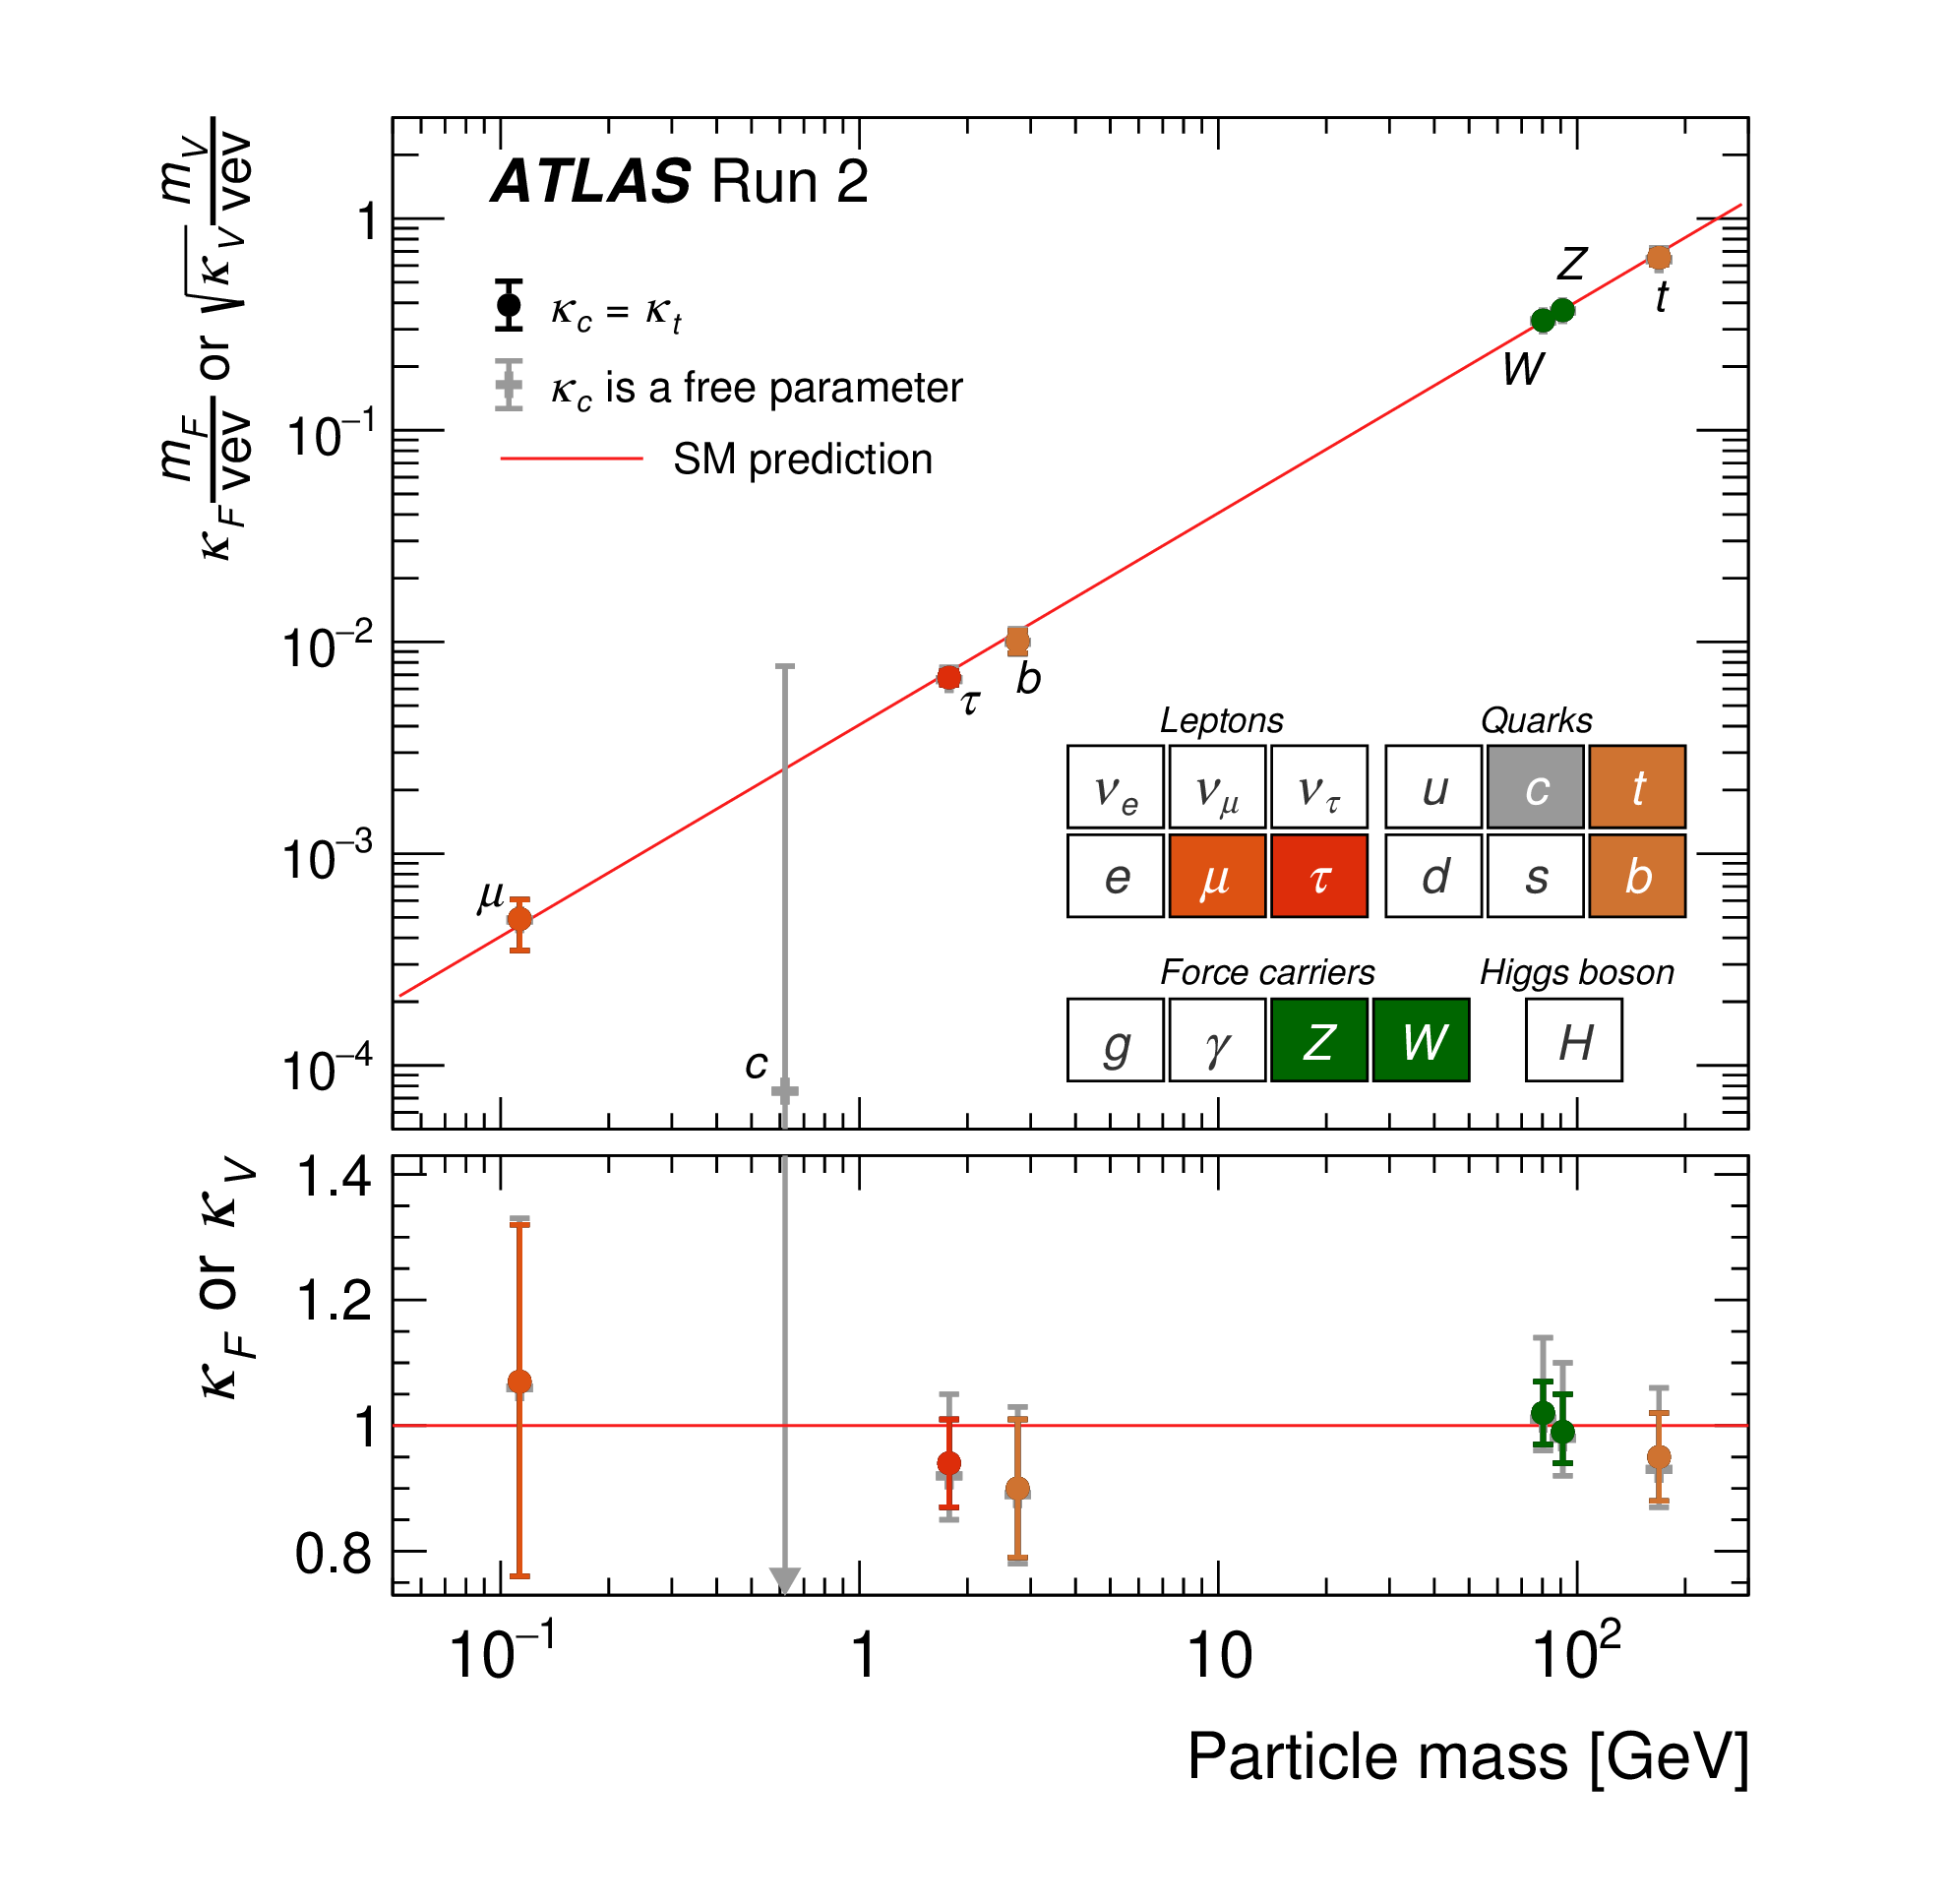
\includegraphics[width=0.6\linewidth]{figures/chapter2/higgs_couplings.png}
	\caption{Reduced Higgs boson coupling strength modifiers as a function of particle mass, measured
	by ATLAS with the full Run 2 dataset~\cite{ATLASHiggsTenYears}. The red line shows the SM
	prediction that the Higgs coupling scales linearly with mass. % TODO: replace cite key ATLASHiggsTenYears with correct key for arXiv:2207.00092
	}
	\label{fig:HiggsCouplings}
\end{figure}

\newpage

% ============================================================
% SECTION 2.4 — HIGGS PRODUCTION AND DECAY AT THE LHC
% ------------------------------------------------------------
% ANSWERS: The Higgs boson is predicted by the mechanism above.
%          This section establishes that it has been discovered
%          and describes how it is produced and measured at the LHC.
% LEAVES OPEN: The SM makes specific predictions for all Higgs
%              couplings. Are there BSM deviations? In particular,
%              can we access second-generation Yukawa couplings?
% ============================================================

\section{Higgs Production and Decay at the LHC}
\label{sec:higgs_production}

% ------------------------------------------------------------
% OUTLINE FOR THIS SECTION:
% Para 1 — Discovery
%   - Higgs boson discovered by ATLAS and CMS in 2012 at sqrt(s) = 7-8 TeV
%   - Observed in H->yy and H->ZZ*->4l channels
%   - m_H ~ 125 GeV confirmed; spin-0, CP-even quantum numbers
%   - All coupling measurements to date consistent with SM
% Para 2 — Production modes
%   - Four main mechanisms: ggF, VBF, VH, ttH (reference fig:HiggsProduction)
%   - Cross sections at 13 TeV: ggF ~50 pb, VBF ~4 pb, VH ~2.5 pb, ttH ~0.5 pb
%   - Reference fig:HiggsXSvsSqrts for energy dependence
%   - Clean up "Hanbook" typo -> cite LHCHiggsXSWG4 properly
% Para 3 — Decay channels and VH strategy
%   - Branching ratios: H->bb ~58%, H->cc ~2.9%, others (reference fig:HiggsBranchingRatios)
%   - H->bb and H->cc overwhelmed by QCD multijet background in inclusive searches
%   - VH production provides leptonic W/Z decay as trigger -> suppresses background
%   - H->cc not yet observed; VH(H->cc) is the charm Yukawa target of this thesis
% ------------------------------------------------------------

% NOTE: Bare URL on line below needs to become a \cite{} once bib entry is added.
% LHC Higgs XS WG Yellow Report 4: https://arxiv.org/abs/1610.07922
% ATLAS discovery: https://arxiv.org/abs/1207.7214
% CMS discovery: https://arxiv.org/abs/1207.7235

% TODO: Add ATLAS and CMS discovery figures here (or move to Chapter 1 introduction
%       if Chapter 1 serves as physics motivation). The H->yy invariant mass peak
%       and H->ZZ*->4l mass spectrum are iconic figures that motivate the program.

% TODO: Rewrite this opening paragraph. It re-explains the Higgs mechanism
%       and SSB which is already covered in Section 2.2. This paragraph should
%       instead open with the 2012 discovery and move directly into production/decay.
%       Draft: "The Higgs boson was discovered by ATLAS and CMS in 2012 using
%       ~10 fb^-1 at sqrt(s)=7-8 TeV, observed in the H->yy and H->ZZ*->4l
%       channels. Its mass was measured to be m_H ~ 125 GeV, and subsequent
%       measurements confirmed spin-0 and CP-even quantum numbers consistent
%       with the SM. All coupling measurements to date are consistent with SM
%       predictions."
A landmark achievement in experimental particle physics was obtained at the LHC in 2012 with the discovery of the Higgs Boson. This particle is a quantization of the Higgs field which is responsible for mass generation in the standard model, which up until then was a crucial missing piece. The Higgs field has a wine bottle shape that leads to spontaneous symmetry breaking which is a crucial part of the Higgs mechanism giving rise to the mass of vector bosons. Since its discovery, many of the Higgs properties have been studied including its mass, spin, coupling to gauge bosons, and coupling to third generation fermions. As of date, all experimental observations are in line with the Standard Model predictions.

\begin{figure}[h]
	\centering
	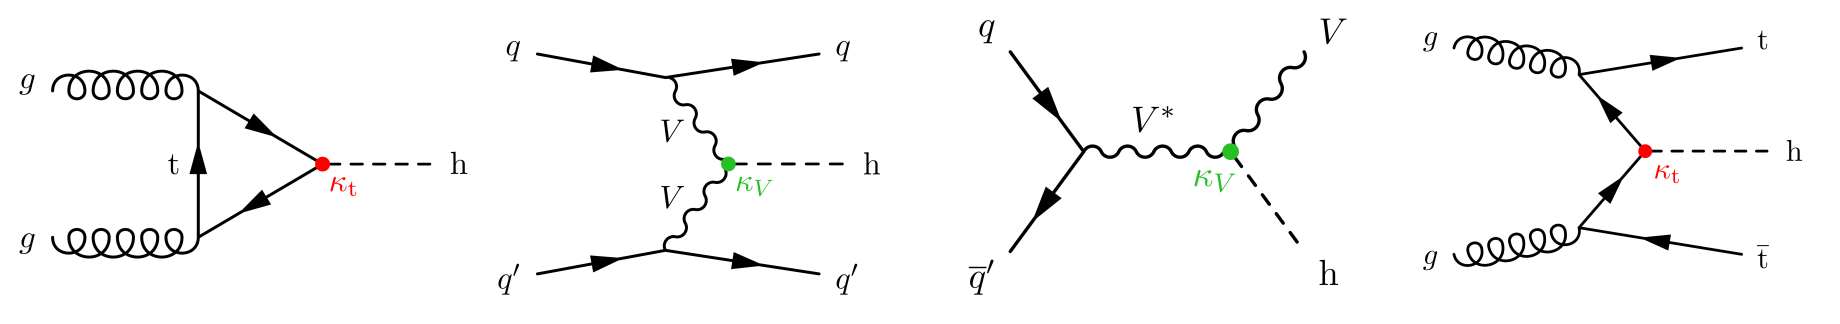
\includegraphics[width=\linewidth]{figures/chapter2/Higgs_Production.png}
	\caption{% TODO: Add caption. Suggest: "Feynman diagrams for the four main
	% Higgs boson production modes at the LHC: gluon-gluon fusion (ggF),
	% vector boson fusion (VBF), associated production (VH), and top quark
	% associated production (ttH)."}
	\label{fig:HiggsProduction}
\end{figure}

% TODO: "Hanbook" -> "LHC Higgs Cross Section Working Group Yellow Report" (fix typo and wording)
The Higgs boson has four unique production modes, shown in Figure \ref{fig:HiggsProduction}. In current LHC conditions with a center of mass energy at 13 TeV, the Hanbook of LHC Higgs cross section \cite{LHCHiggsXSWG4} shows that $\sigma_{ggF} \approx 50 pb$, $\sigma_{VBF} \approx 4pb$, $\sigma_{VH} \approx 2.5 pb$, and $\sigma_{ttH} \approx 0.5 pb$. Each of these channels has their own unique backgrounds. The branching ratio of the Higgs boson decays is shown in Figure \ref{fig:HiggsBranchingRatios}. Notice the largest branching ratio is $H \rightarrow bb$ at around 58\%. Unfortunately, to take advantage of this channel an analysis will need to suppress the dominant hadronic multi-jet background at the LHC. Currently, ATLAS has focused large efforts on the VH channel, as it allows leptonic channels originating from the associated vector boson decay.

\begin{figure}[h]
	\centering
	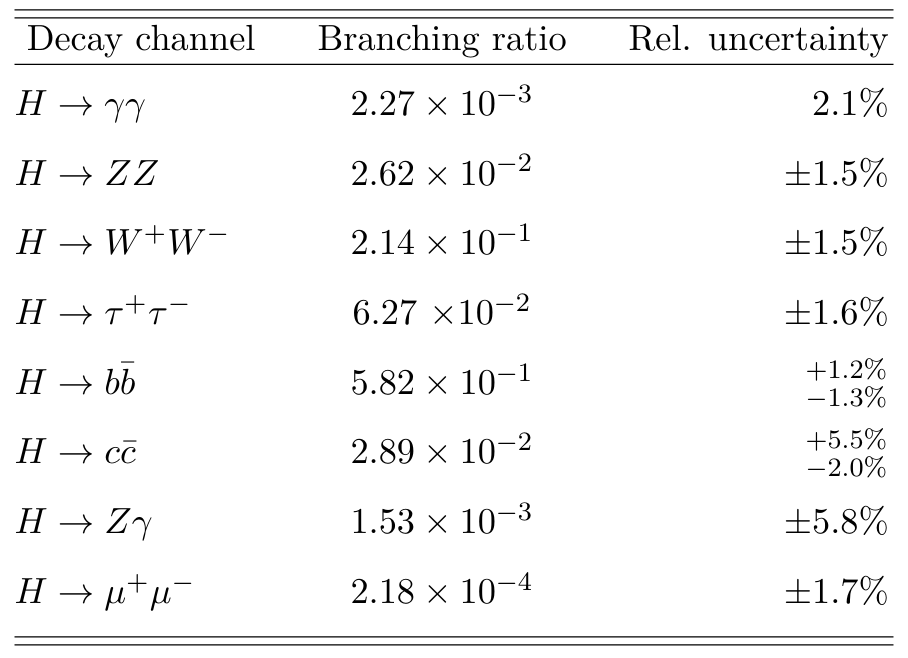
\includegraphics[width=0.4\linewidth]{figures/chapter2/Higgs_Branching_Ratios.png}
	\caption{% TODO: Add caption. Suggest: "SM Higgs boson branching ratios as a
	% function of m_H~\cite{LHCHiggsXSWG4}. The dominant decay is H->bb at ~58%.
	% The H->cc branching ratio is ~2.9% and has not yet been observed directly."}
	\label{fig:HiggsBranchingRatios}
\end{figure}

\begin{itemize}
  \item ATLAS and CMS observed a new boson at $m_H \approx 125$ GeV in 2012 via the $H \rightarrow \gamma\gamma$ and $H \rightarrow ZZ^* \rightarrow 4\ell$ channels~\cite{ATLASDiscovery,CMSDiscovery}. Subsequent measurements confirmed spin-0 and CP-even quantum numbers.
  % ~5 fb^-1 at 7 TeV + ~5 fb^-1 at 8 TeV; ATLAS arXiv:1207.7214, CMS arXiv:1207.7235
  \item The VH production mode is experimentally favorable for hadronic Higgs decays: the leptonic $W$ or $Z$ decay provides a clean trigger and suppresses QCD multijet backgrounds.
  % ggF largest cross section but no additional hard objects; VBF has two forward jets; ttH has ttbar pair
  \item $H \rightarrow c\bar{c}$ has not yet been observed. This analysis targets $VH(H \rightarrow c\bar{c})$ as a direct probe of the charm Yukawa coupling.
  \item FIGURE: ATLAS and CMS discovery plots ($H \rightarrow \gamma\gamma$ invariant mass peak,
  %   $H \rightarrow ZZ^* \rightarrow 4\ell$ mass spectrum).
  %   Move to Chapter 1 if that chapter serves as physics motivation.
  %
  %   ATLAS paper page (HIGG-2012-27): https://atlas.web.cern.ch/Atlas/GROUPS/PHYSICS/PAPERS/HIGG-2012-27/
  %     H->yy:    fig_004.png / fig_004.pdf  (diphoton invariant mass, combined 7+8 TeV)
  %     H->ZZ*4l: fig_002.png / fig_002.pdf  (four-lepton invariant mass, 80-250 GeV range)
  %     arXiv: 1207.7214
  %
  %   CMS paper page (HIG-12-028): https://cms-results.web.cern.ch/cms-results/public-results/publications/HIG-12-028/
  %     H->yy:    CMS-HIG-12-028_Figure_003.png / .pdf  (diphoton invariant mass with signal+background fit)
  %     H->ZZ*4l: CMS-HIG-12-028_Figure_004.png / .pdf  (four-lepton invariant mass)
  %     arXiv: 1207.7235
  %
  % SOURCE for cross section figure: LHC Higgs XS WG 2014
  %   direct URL: https://twiki.cern.ch/twiki/pub/LHCPhysics/LHCHWGCrossSectionsFigures/7-14.xsec.pdf
  %   Reference: LHC Higgs XS WG Yellow Report 4, arXiv:1610.07922
\end{itemize}

\begin{figure}[h]
	\centering
	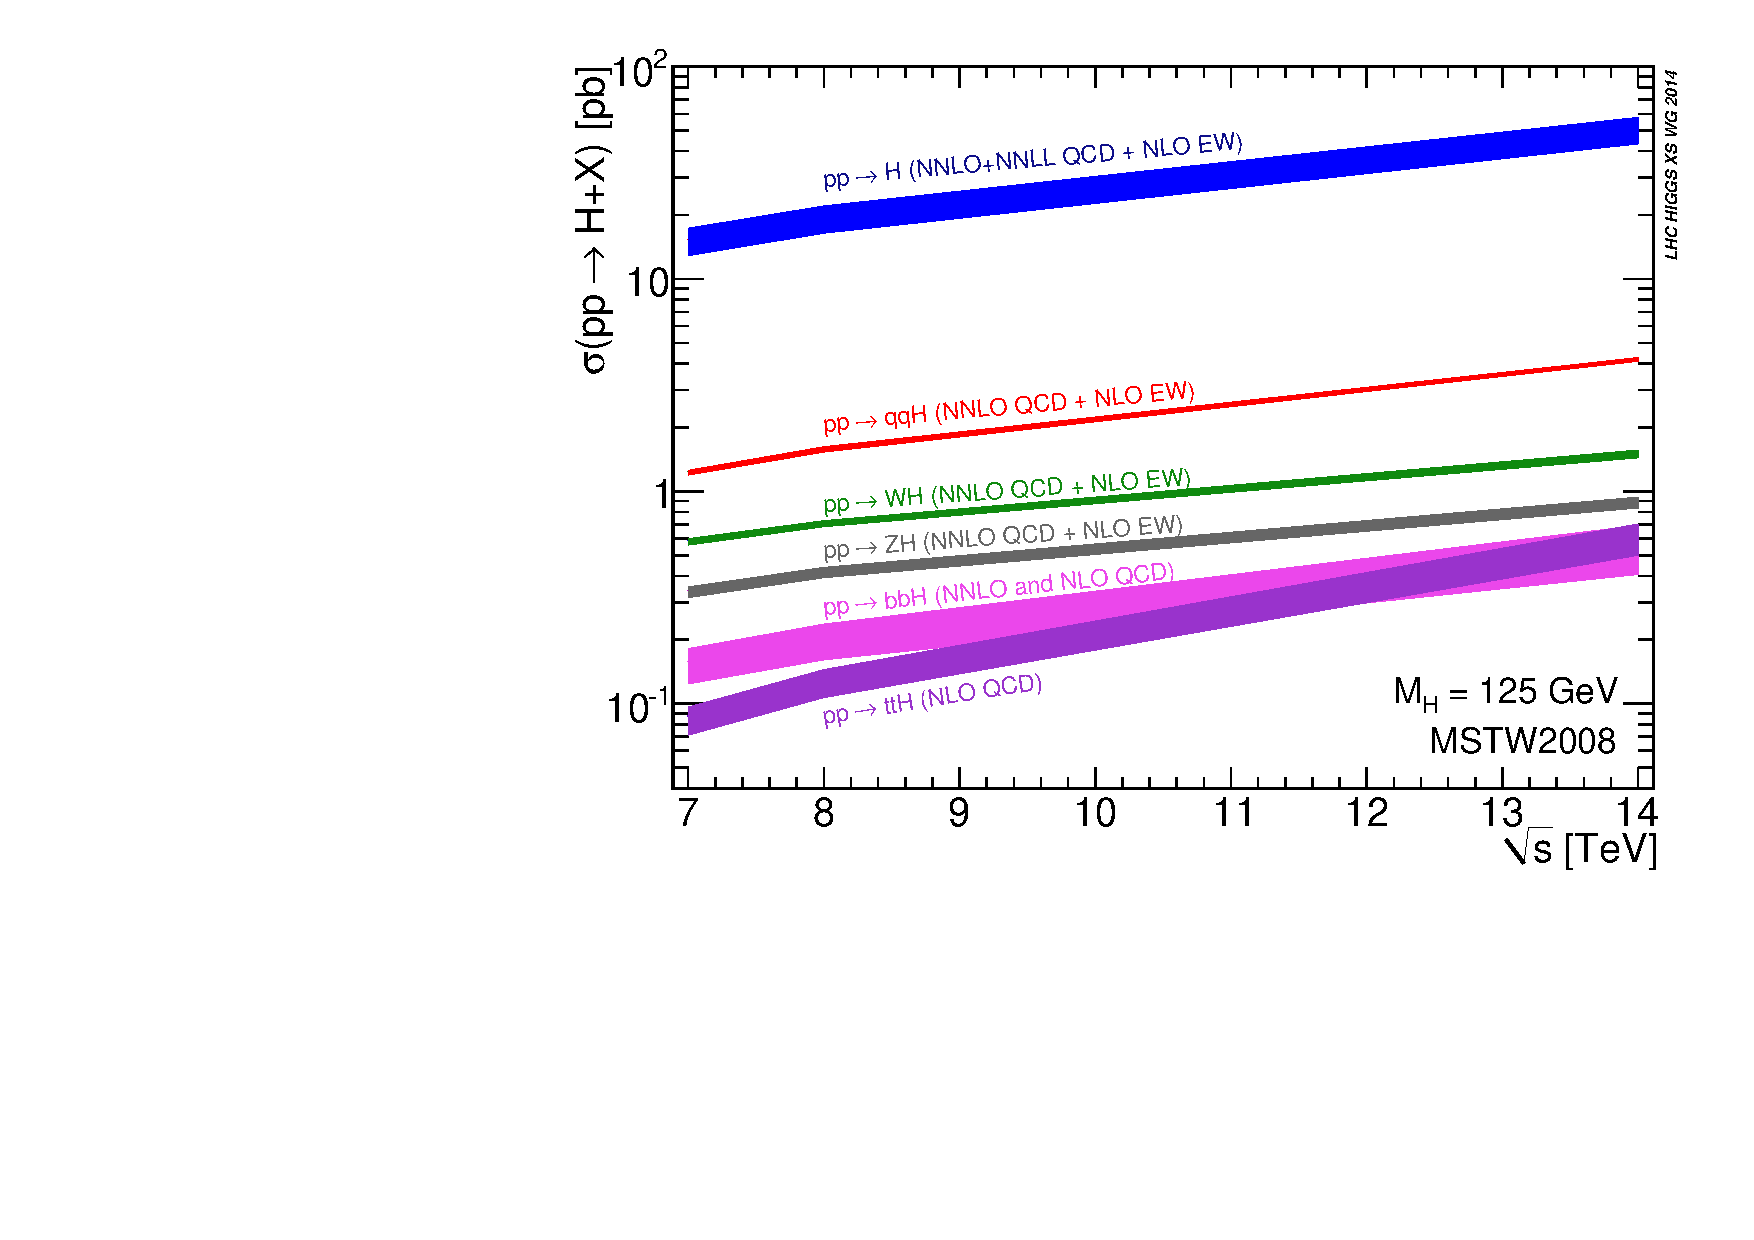
\includegraphics[width=0.6\linewidth]{figures/chapter2/Higgs_XS_vs_sqrts.pdf}
	\caption{SM Higgs boson production cross sections as a function of centre-of-mass energy
	$\sqrt{s}$ for $m_H = 125$ GeV~\cite{LHCHiggsXSWG4}. Gluon fusion ($pp \rightarrow H$)
	dominates across all energies. Vector boson fusion ($pp \rightarrow qqH$), associated
	production ($WH$, $ZH$), and $t\bar{t}H$ follow in decreasing order. Bands indicate
	theoretical uncertainties.}
	\label{fig:HiggsXSvsSqrts}
\end{figure}

\newpage

% ============================================================
% SECTION 2.5 — OPEN QUESTIONS
% ------------------------------------------------------------
% ANSWERS: The LHC has confirmed SM Higgs couplings to third-
%          generation fermions and gauge bosons. But the SM
%          itself has deeper unresolved problems that motivate
%          a continued precision measurement program.
% SETS UP: The thesis analysis as a contribution to this program.
% ============================================================

\section{Open Questions}
\label{sec:open_questions}

% ------------------------------------------------------------
% OUTLINE FOR THIS SECTION:
% Para 1 — Hierarchy problem
%   - Large disparity between electroweak scale (~100 GeV) and Planck scale (~10^19 GeV)
%   - Quantum corrections drive m_H to Planck scale without fine-tuned cancellation
%   - Top quark loop is the dominant correction (coefficient ~ y_t^2 ~ 1)
%   - BSM theories (e.g. SUSY) predict top partner near TeV scale to cancel correction
% Para 2 — EW vacuum stability
%   - Measured m_H ~ 125 GeV and m_t ~ 173 GeV place SM vacuum in metastable region
%   - Universe may reside in a false vacuum (cite Buttazzo et al.)
%   - Optional: include EW vacuum stability phase diagram (fig commented out below)
% Para 3 — Other open questions and connection to thesis
%   - SM has no explanation for matter-antimatter asymmetry, dark matter, dark energy
%   - Three-generation structure unexplained (flagged in Section 2.1)
%   - Connect to thesis contributions:
%       * VH(H->cc): direct probe of unmeasured charm Yukawa coupling
%       * Pileup mitigation: enabling precision measurements at HL-LHC
%       * Top polarimetry: probing quantum entanglement in tt̄ production
% ------------------------------------------------------------

\begin{itemize}
  \item The SM does not describe gravity, dark matter, or the matter-antimatter asymmetry of the universe.
  \item The hierarchy problem: quantum corrections drive $m_H$ toward the Planck scale, requiring fine-tuned cancellation unless new physics exists at the TeV scale. The dominant contribution to these corrections comes from the top quark loop, which enters with a coefficient proportional to $y_t^2$. Because $y_t \approx 1$ is so large compared to all other SM fermion Yukawa couplings, the top quark is responsible for the largest single quantum correction to the Higgs mass. This is why many BSM theories targeting the hierarchy problem, such as supersymmetry, predict a top quark superpartner near the TeV scale.
  \item EW vacuum stability: the measured $m_H$ and $m_t$ place the vacuum in a metastable region, suggesting the universe may reside in a false vacuum~\cite{Buttazzo:2013uya}.
  % Yukawa coupling hierarchy (three generations, large mass spread) also unexplained by SM.
  % HL-LHC will probe second-generation Yukawa couplings at O(10%) precision.
  %\item FIGURE: EW vacuum stability phase diagram (top pole mass $M_t$ vs Higgs pole mass $M_h$),
  %   showing stability, meta-stability, and instability regions. The right panel zooms into
  %   the experimentally measured region, with 1, 2, 3$\sigma$ contours showing the measured
  %   $M_h$ and $M_t$ values sit in the meta-stable region near the stability boundary.
  %
  %   SOURCE: Buttazzo et al., arXiv:1307.3536
  %     "Investigating the near-criticality of the Higgs boson"
  %     Buttazzo, Degrassi, Giardino, Giudice, Sala, Salvio, Strumia (2013)
  %     Figure 3 (Left panel preferred; or use both Left+Right as a combined figure)
  %     x-axis: Higgs pole mass $M_h$ in GeV (0-200 GeV, zoom 120-132 GeV)
  %     y-axis: Top pole mass $M_t$ in GeV (0-200 GeV, zoom 168-180 GeV)
  %     Regions: Stability (green), Meta-stability (yellow), Instability (red)
  %     Dotted contours show instability scale $\Lambda_I$ in GeV
  %     Full caption from paper: "SM phase diagram in terms of Higgs and top pole masses.
  %       The plane is divided into regions of absolute stability, meta-stability, instability
  %       of the SM vacuum, and non-perturbativity of the Higgs quartic coupling."
\end{itemize}
